\documentclass[11pt]{article}
\usepackage[margin=1in]{geometry}
\usepackage{graphicx}
\usepackage{booktabs}
\usepackage{float}
\usepackage{hyperref}
\usepackage{setspace}
\setstretch{1.05}
\title{CMPS261 Project Report}
\author{Jiany Samara \\ Jad Mouawad}
\date{}

\begin{document}
\maketitle

\section{Dataset Exploration and Preprocessing}
We use monthly macroeconomic series from FRED and align them into one reproducible panel.
Core series: CPI, unemployment, interest rate, M2, Treasury 10Y, oil price, PPI, retail sales, sentiment, employment, and housing starts.

Main target in final evaluation is \texttt{target\_yoy\_t\_plus\_1}, i.e., next-month CPI YoY inflation.

Preprocessing steps used:
\begin{enumerate}
  \item load from FRED or cached files
  \item enforce monthly alignment and duplicate checks
  \item construct leakage-safe forecast target (horizon = 1 month)
  \item engineer macro features
  \item build chronological train/val/test split.
\end{enumerate}

Final split used in the report: train 347 rows (to 2021-11-01), validation 24 rows (to 2023-11-01), test 24 rows (2023-12-01 to 2026-01-01).

\begin{figure}[H]
\centering
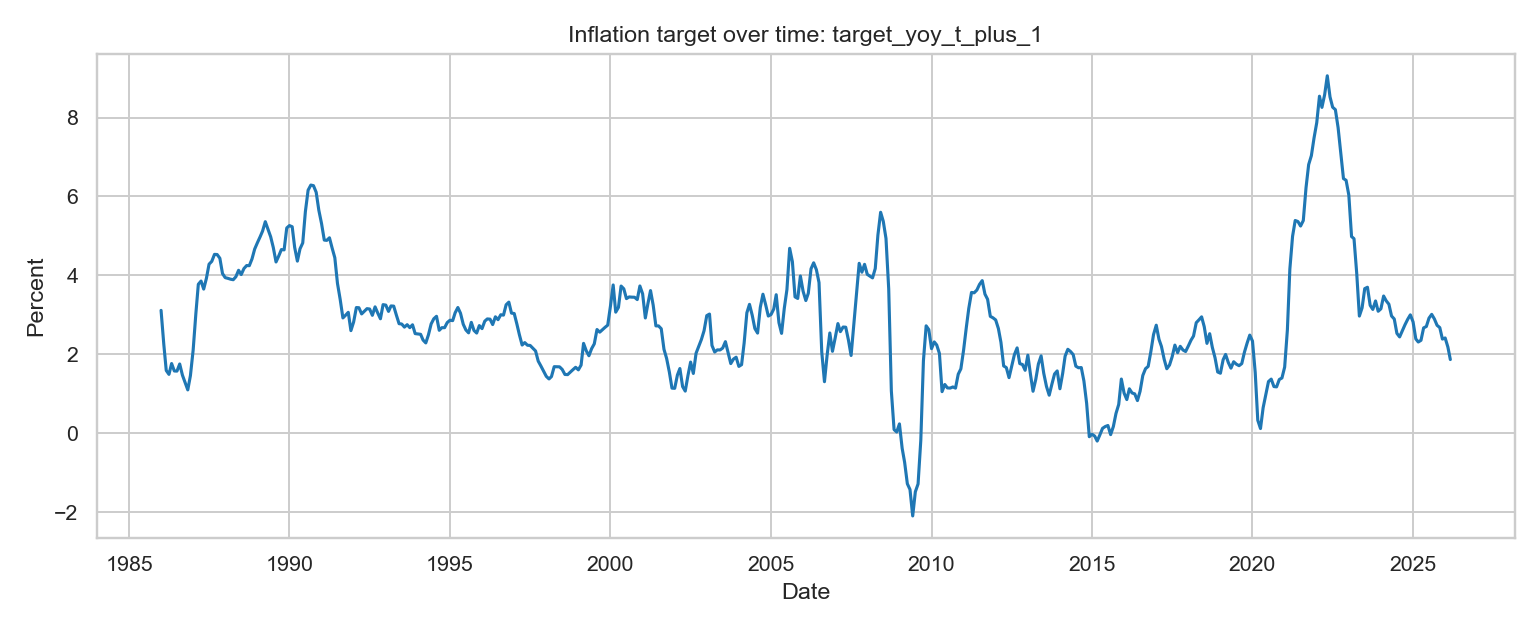
\includegraphics[width=0.82\textwidth]{figures/target_series.png}
\caption{Target series over time.}
\end{figure}

\begin{figure}[H]
\centering
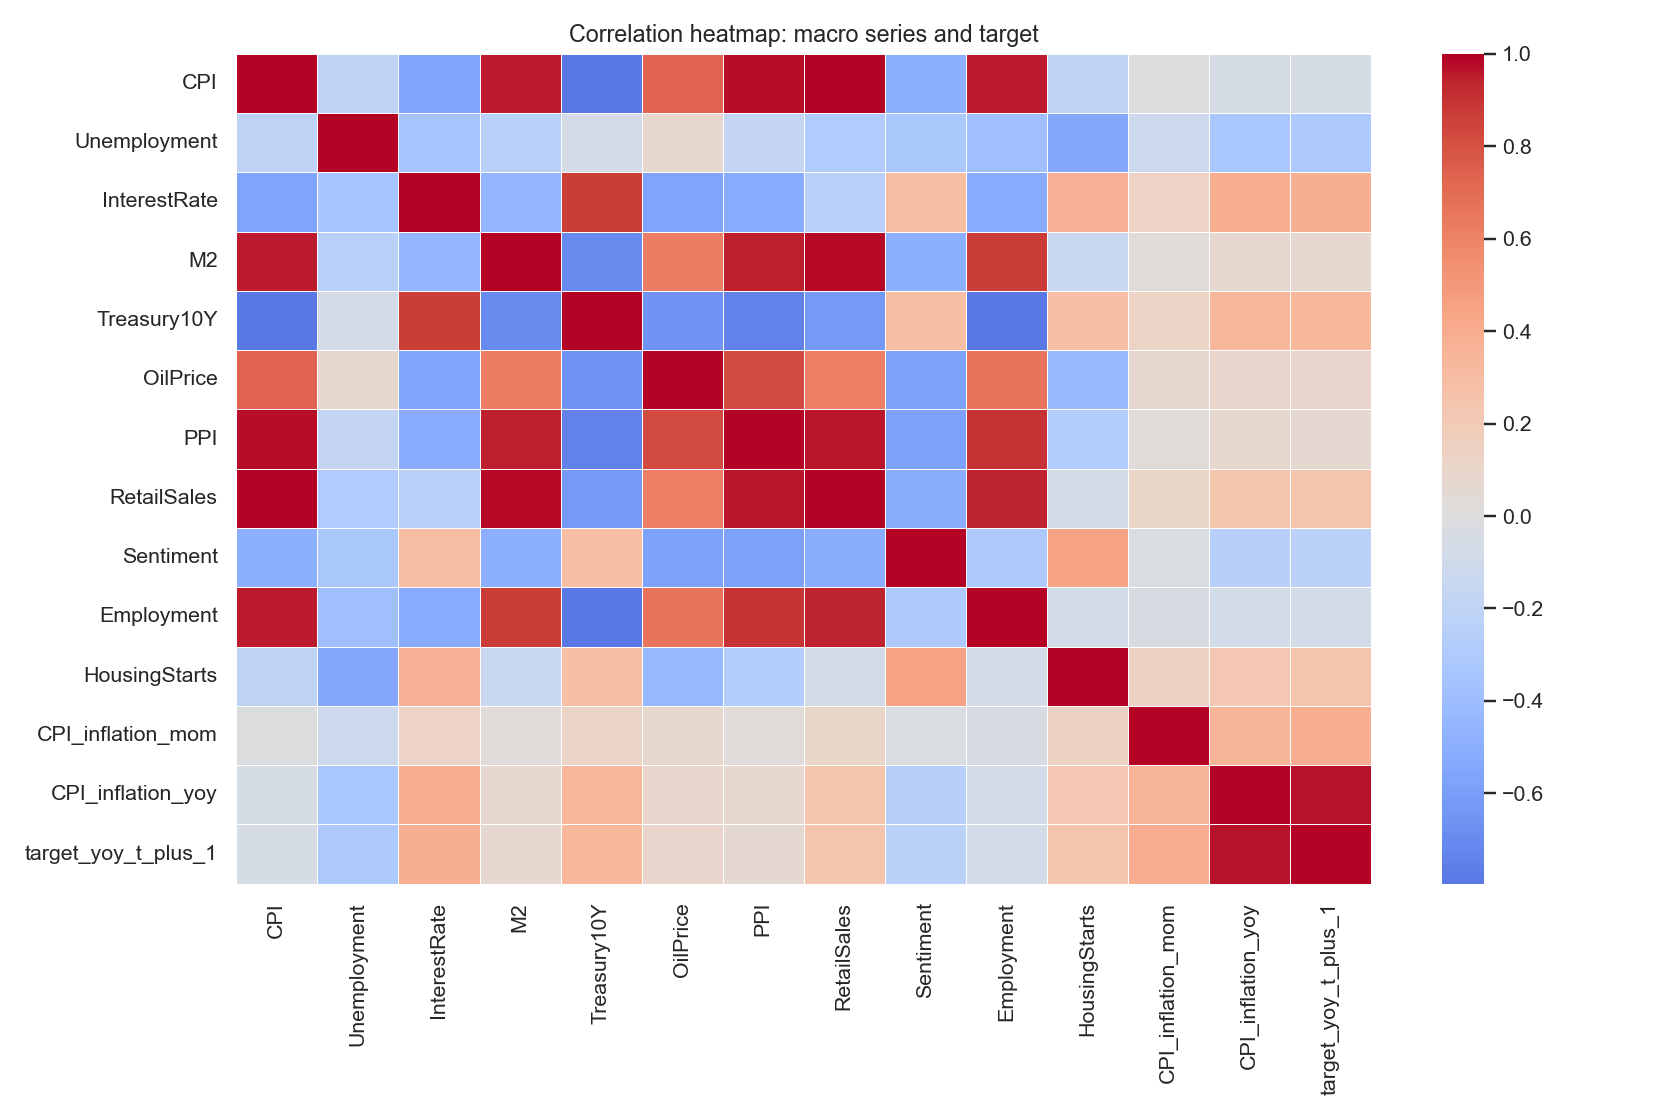
\includegraphics[width=0.82\textwidth]{figures/correlation_heatmap.png}
\caption{Feature correlation heatmap.}
\end{figure}

\section{Methodology}
Workflow is notebook-first and strictly chronological:
\begin{itemize}
  \item feature engineering and split logic
  \item classical baselines
  \item stacked LSTM
  \item XGBoost
  \item rolling backtest and uncertainty diagnostics
  \item ablations and final comparison.
\end{itemize}

Leakage controls:
\begin{itemize}
  \item validation used for model selection
  \item test used only once for final scoring
  \item MASE scale built from in-sample history only
  \item conformal calibration from validation residuals only.
\end{itemize}

\section{Models and Justification}
Models compared:
\begin{itemize}
  \item Classical: Naive, Seasonal Naive, ARIMA, Ridge, Lasso
  \item Neural: stacked LSTM
  \item Tree model: XGBoost
\end{itemize}

Why this set: it gives an honest baseline range, then tests whether more complex models truly add out-of-sample value.

\section{Evaluation Metrics and Results}
Metrics: MAE (primary), sMAPE, MASE.
Held-out test window: 2023-12-01 to 2026-01-01.

\begin{table}[H]
\centering
\begin{tabular}{lccc}
\toprule
Model & MAE & sMAPE & MASE \\
\midrule
XGBoost (mean\_pooled, delta, lag=24) & 0.1584 & 5.7321 & 0.5474 \\
Lasso (mean\_pooled, delta, lag=24) & 0.1663 & 5.9220 & 0.5747 \\
LSTM (delta, lag=24) & 0.1787 & 6.5616 & 0.6176 \\
Naive Last & 0.1787 & 6.3683 & 0.6175 \\
ARIMA(1,0,0) & 0.3161 & 11.0215 & 1.0922 \\
Ridge (mean\_pooled, delta, lag=24) & 0.3234 & 14.4044 & 1.1177 \\
Seasonal Naive & 0.8453 & 24.1892 & 2.9210 \\
\bottomrule
\end{tabular}
\caption{Main held-out comparison (same evaluation window for all models).}
\end{table}

Best final model is XGBoost by all three metrics.
This suggests nonlinear interactions in the macro features matter, and XGBoost was able to use them better than the sequence model in this sample size.
Lasso being close to the top also shows there is still a strong linear signal in the engineered features.

\begin{figure}[H]
\centering
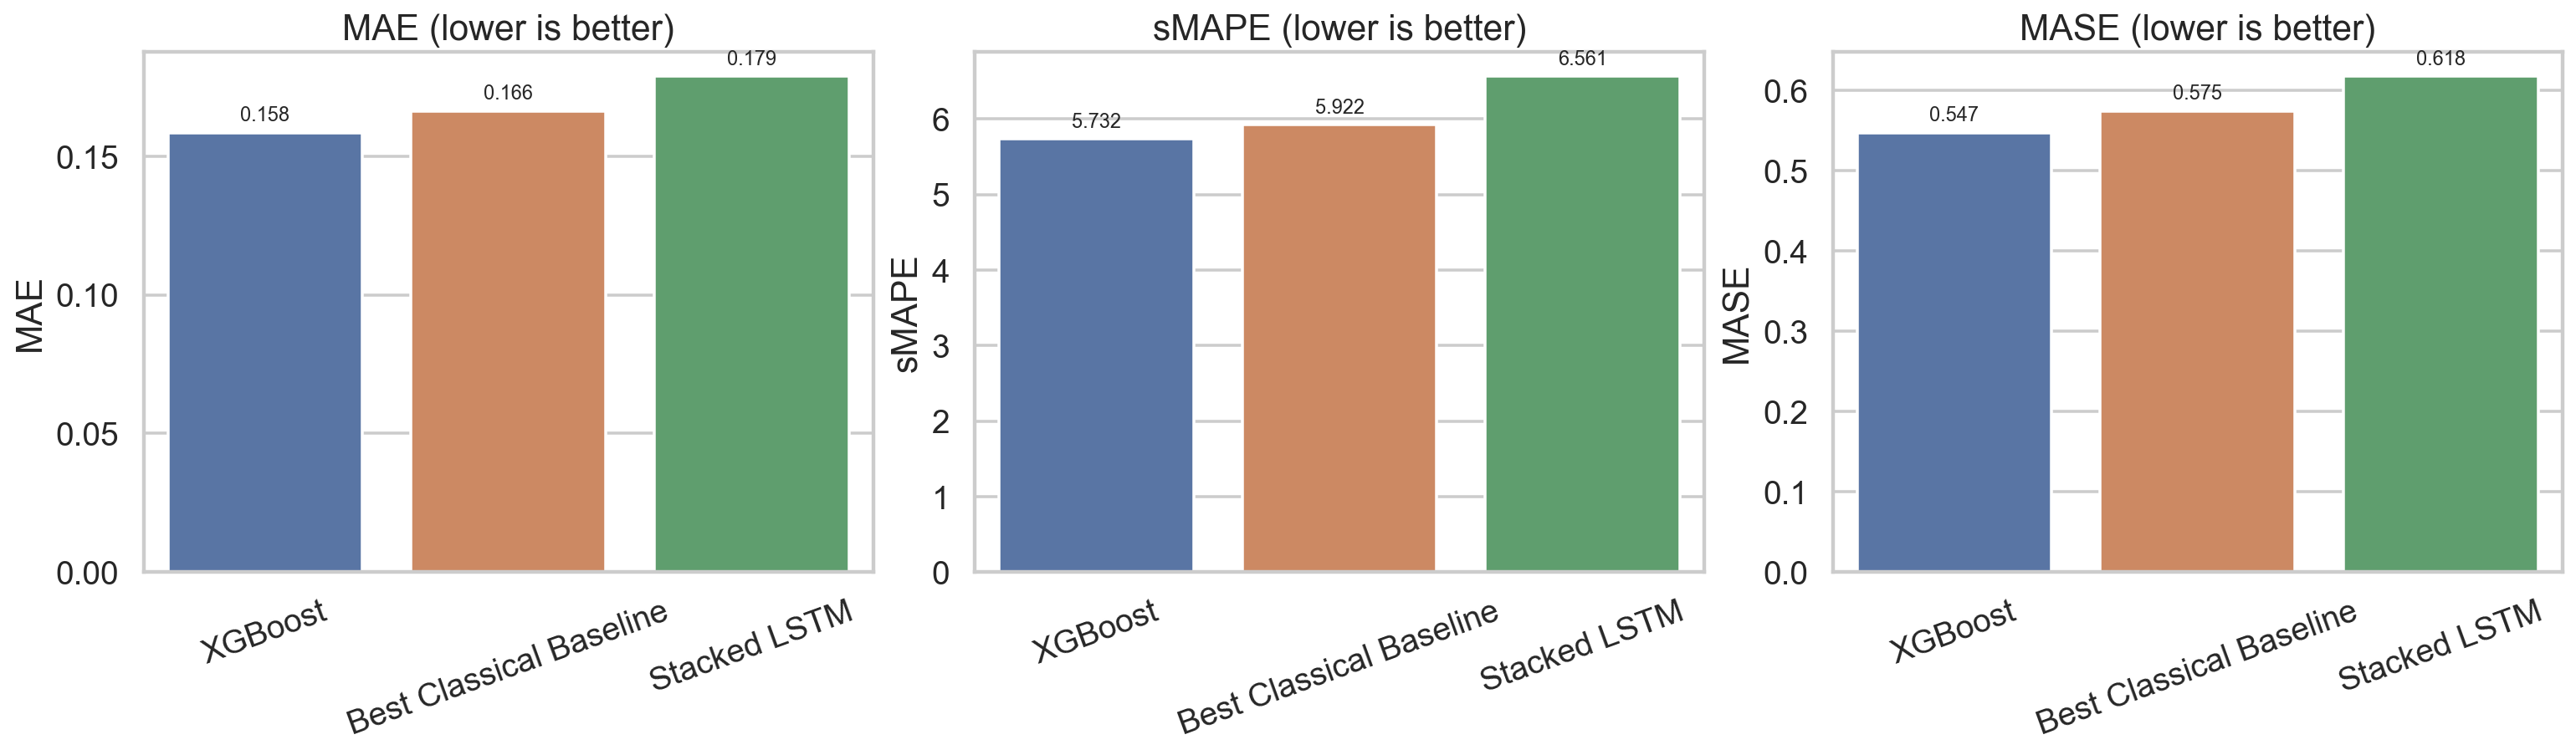
\includegraphics[width=0.88\textwidth]{figures/holdout_metric_comparison.png}
\caption{Hold-out metric comparison.}
\end{figure}

\begin{figure}[H]
\centering
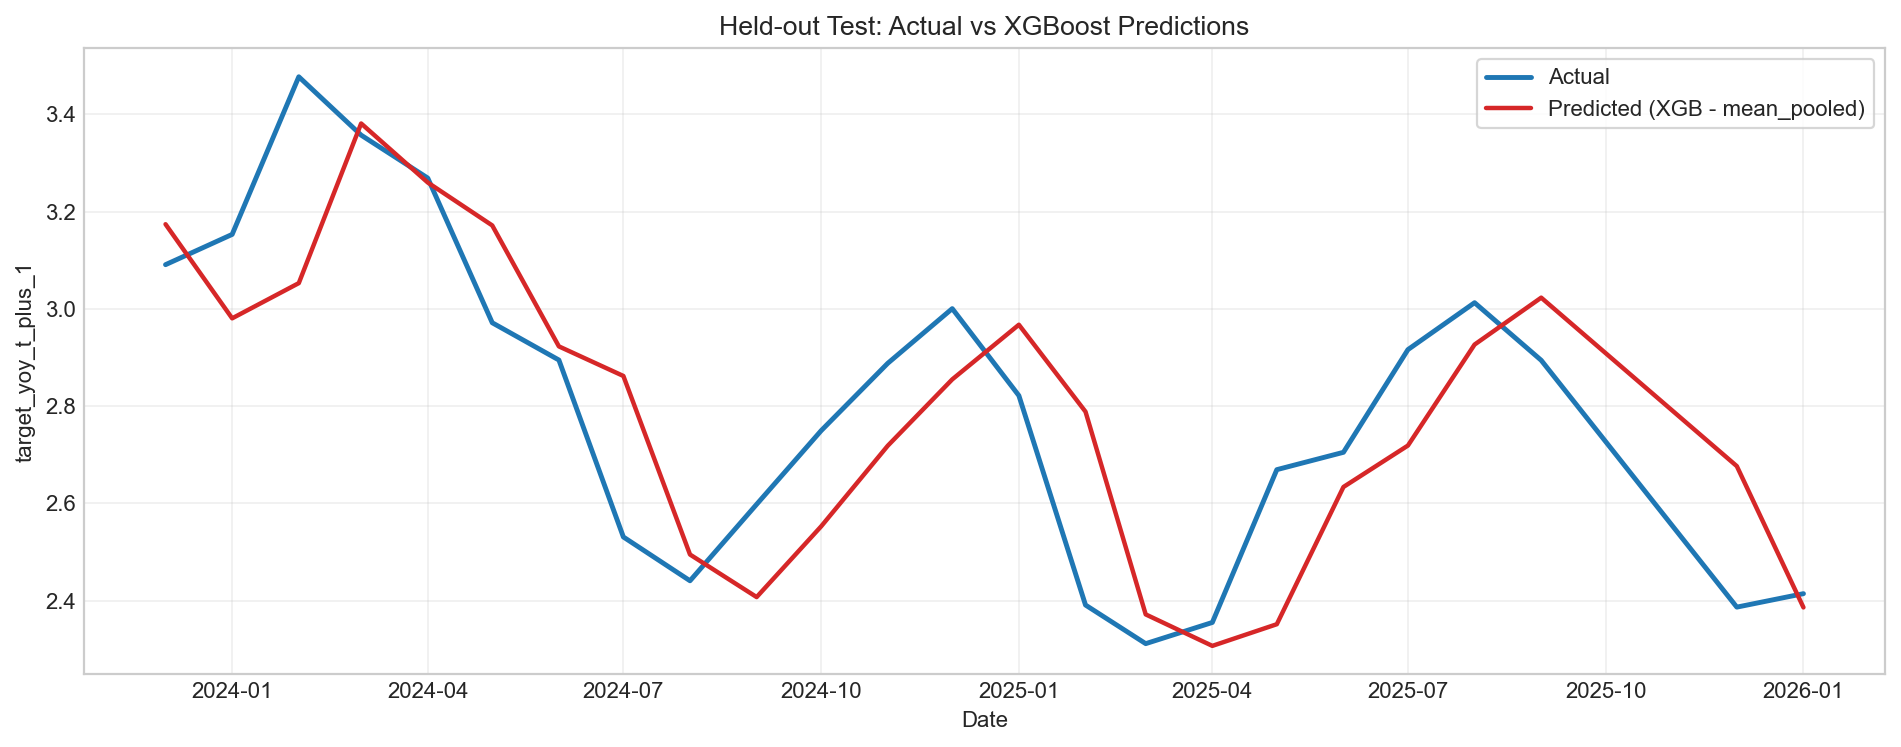
\includegraphics[width=0.88\textwidth]{figures/xgb_actual_vs_pred.png}
\caption{XGBoost: actual vs predicted on held-out test.}
\end{figure}

\begin{figure}[H]
\centering
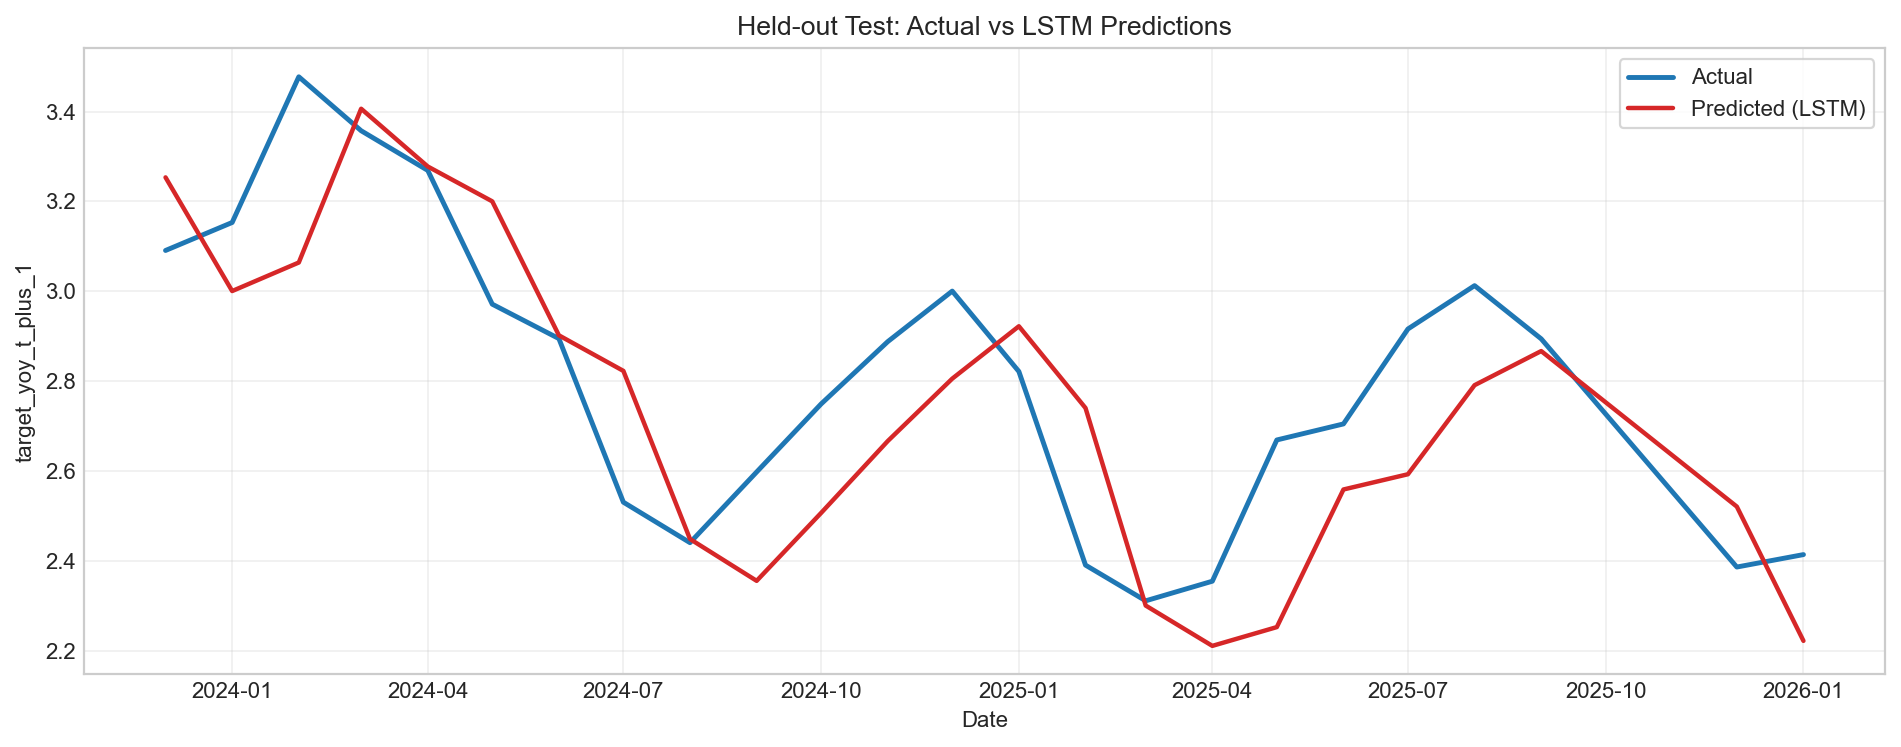
\includegraphics[width=0.88\textwidth]{figures/lstm_actual_vs_pred.png}
\caption{LSTM: actual vs predicted on held-out test.}
\end{figure}

\begin{figure}[H]
\centering
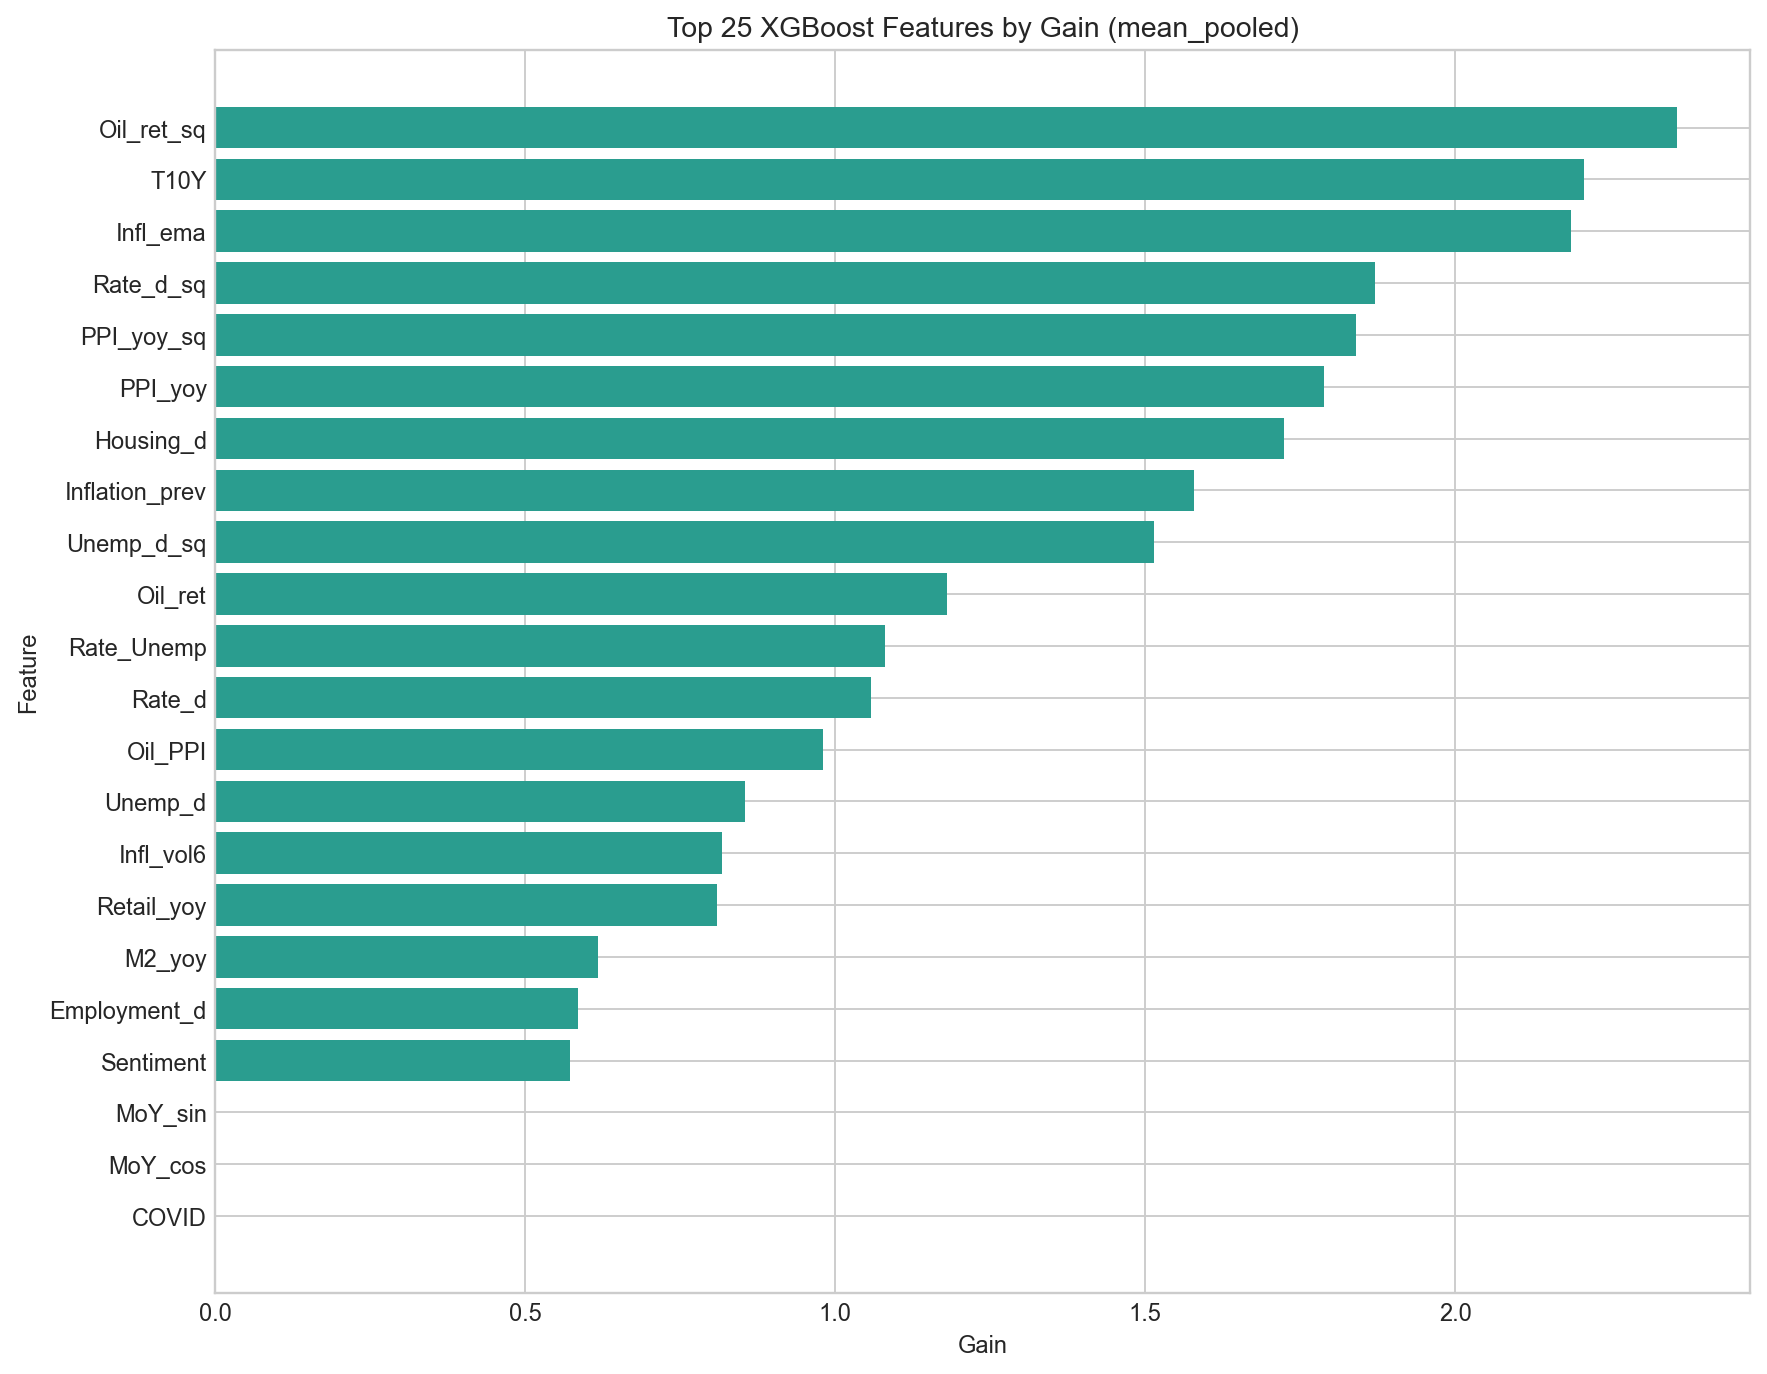
\includegraphics[width=0.72\textwidth]{figures/xgb_feature_importance.png}
\caption{XGBoost feature importance.}
\end{figure}

\noindent \textit{Small note: the COVID dummy was available in training, but it had zero gain in the final XGBoost model. In this split, validation/test are post-COVID, so other macro features carried most of that regime signal.}

\section{Backtest and Uncertainty}
Rolling walk-forward backtest (XGBoost, 25 windows): MAE 0.2946, sMAPE 13.3662, MASE 1.4372.
Compared to the single hold-out test, the rolling scores are weaker, which indicates performance changes across different macro regimes.

Uncertainty diagnostics (LSTM):
\begin{itemize}
  \item MC-dropout coverage: 0.625 (under nominal 0.90)
  \item split-conformal coverage: 1.000 (over nominal 0.90)
\end{itemize}
So the MC-dropout intervals are too narrow, while conformal intervals are conservative on this period.

\begin{figure}[H]
\centering
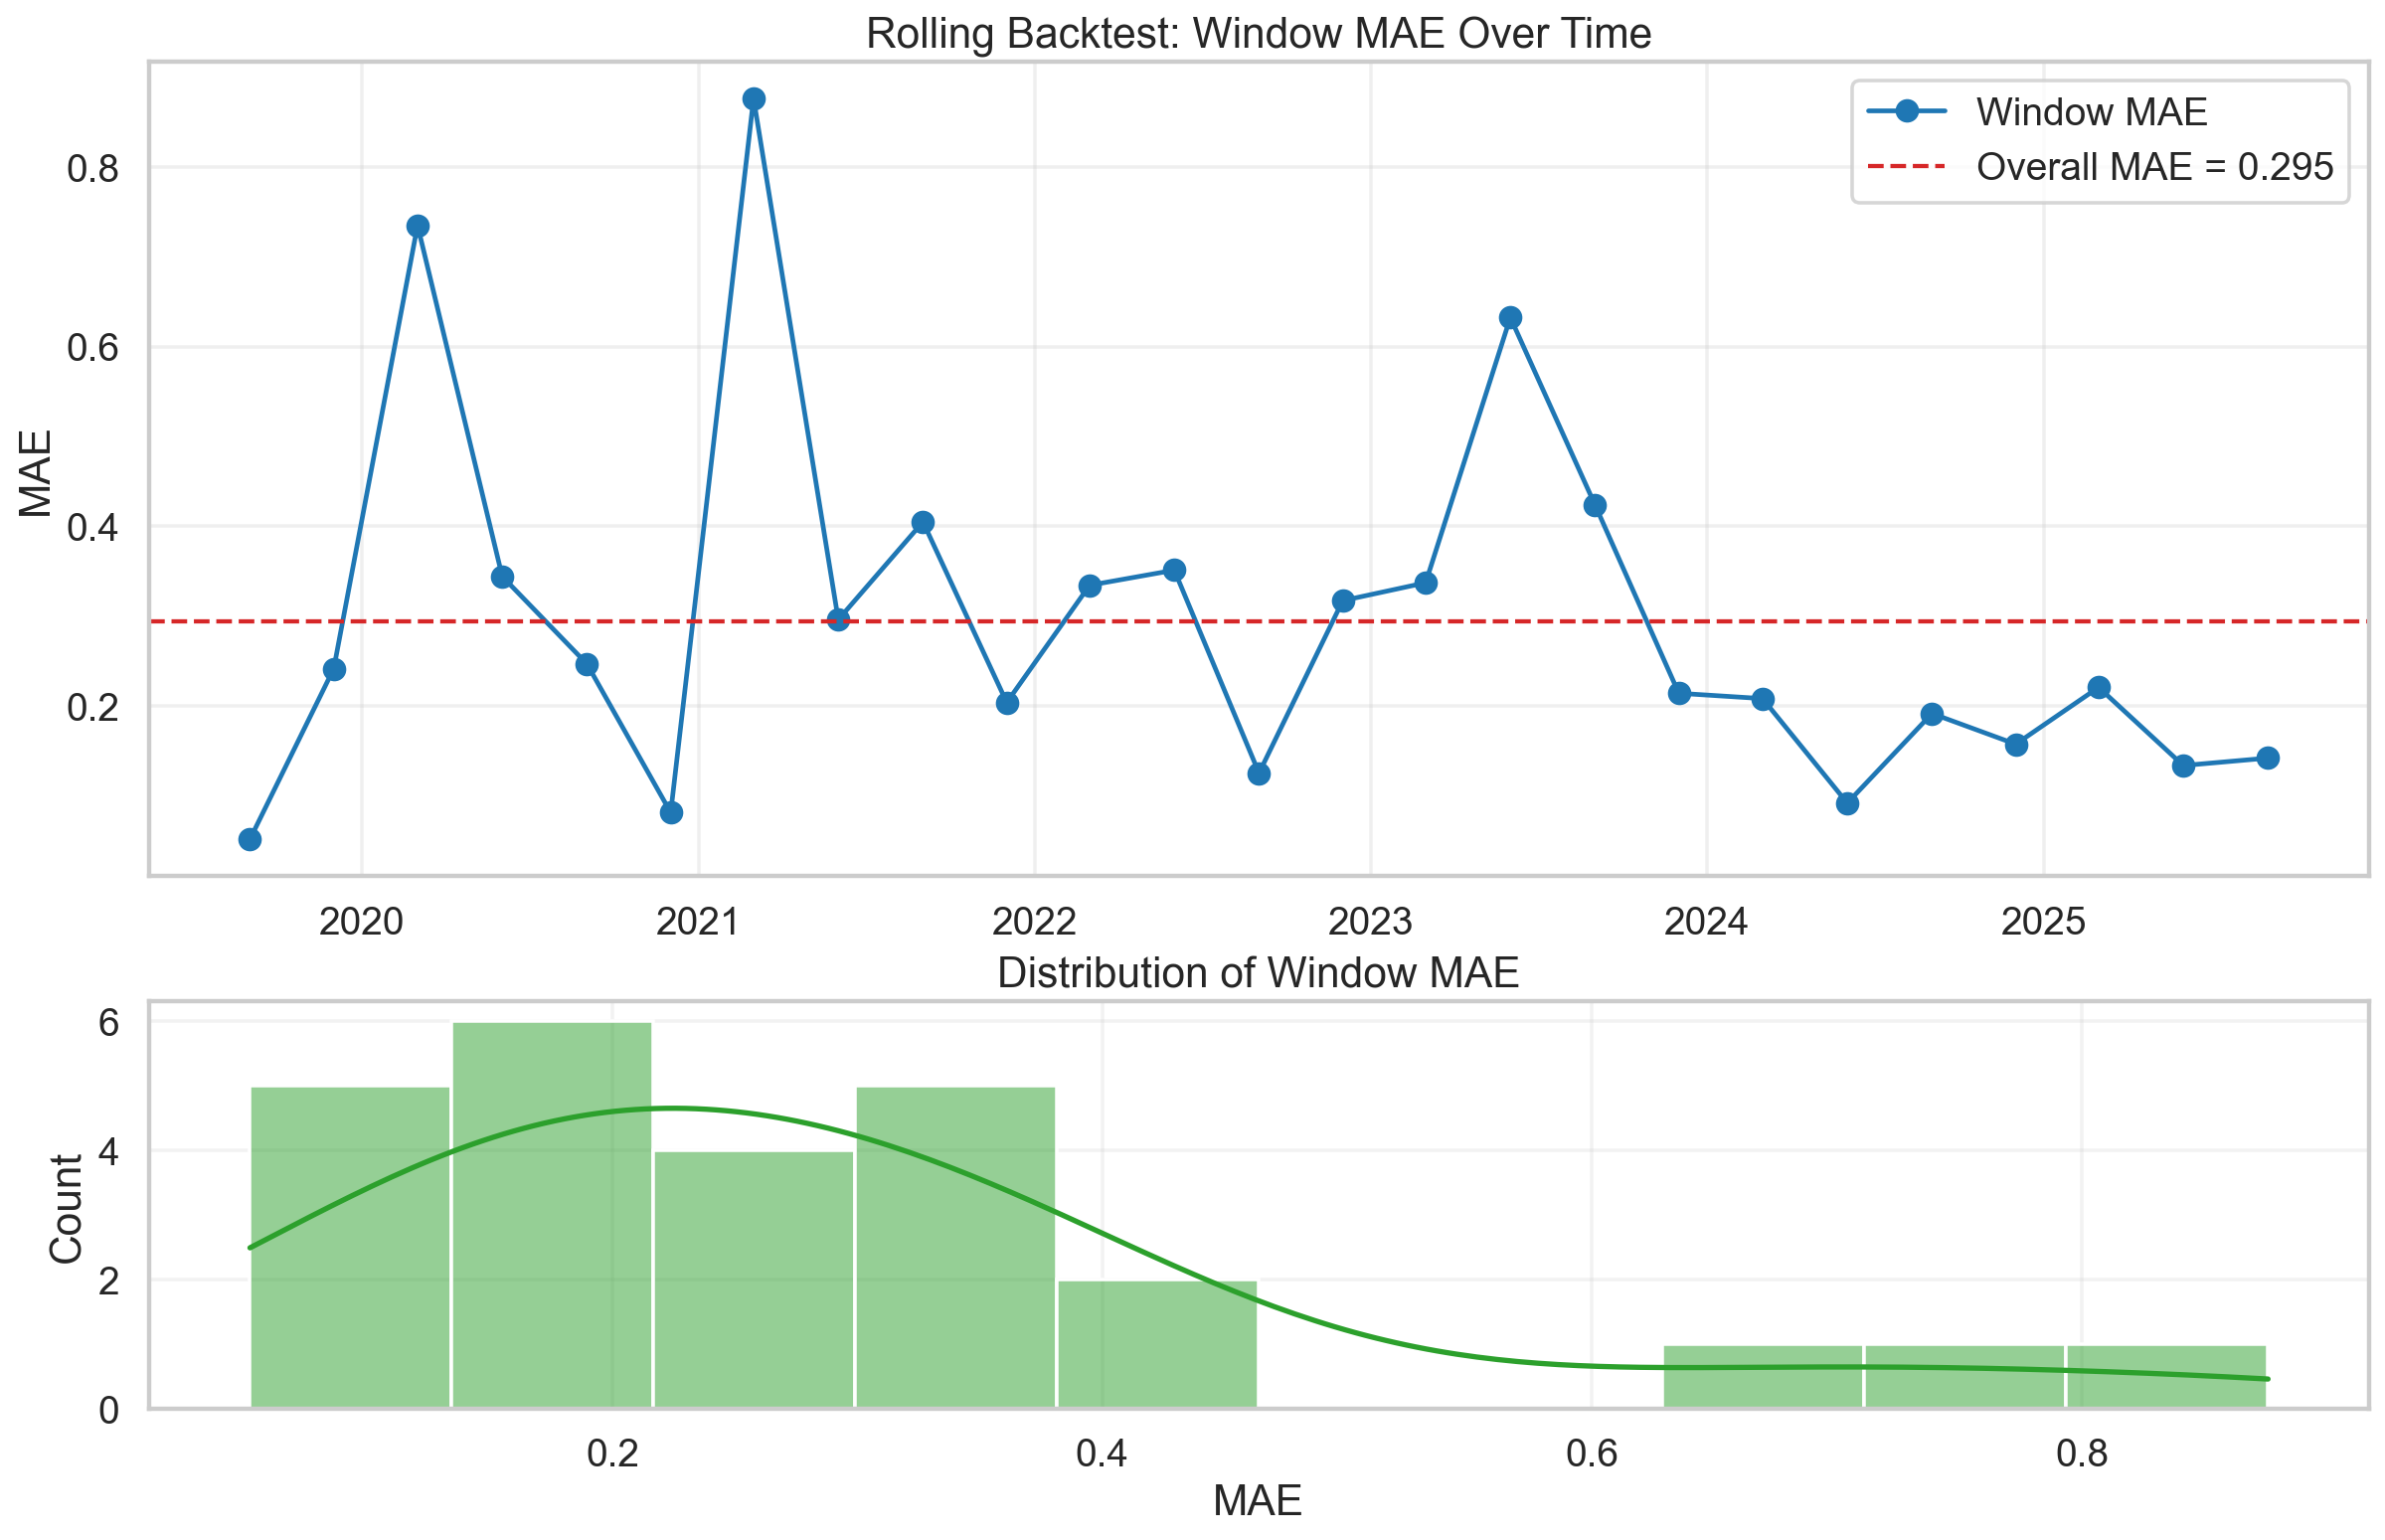
\includegraphics[width=0.74\textwidth]{figures/rolling_backtest_summary.png}
\caption{Rolling backtest summary across windows.}
\end{figure}

\begin{figure}[H]
\centering
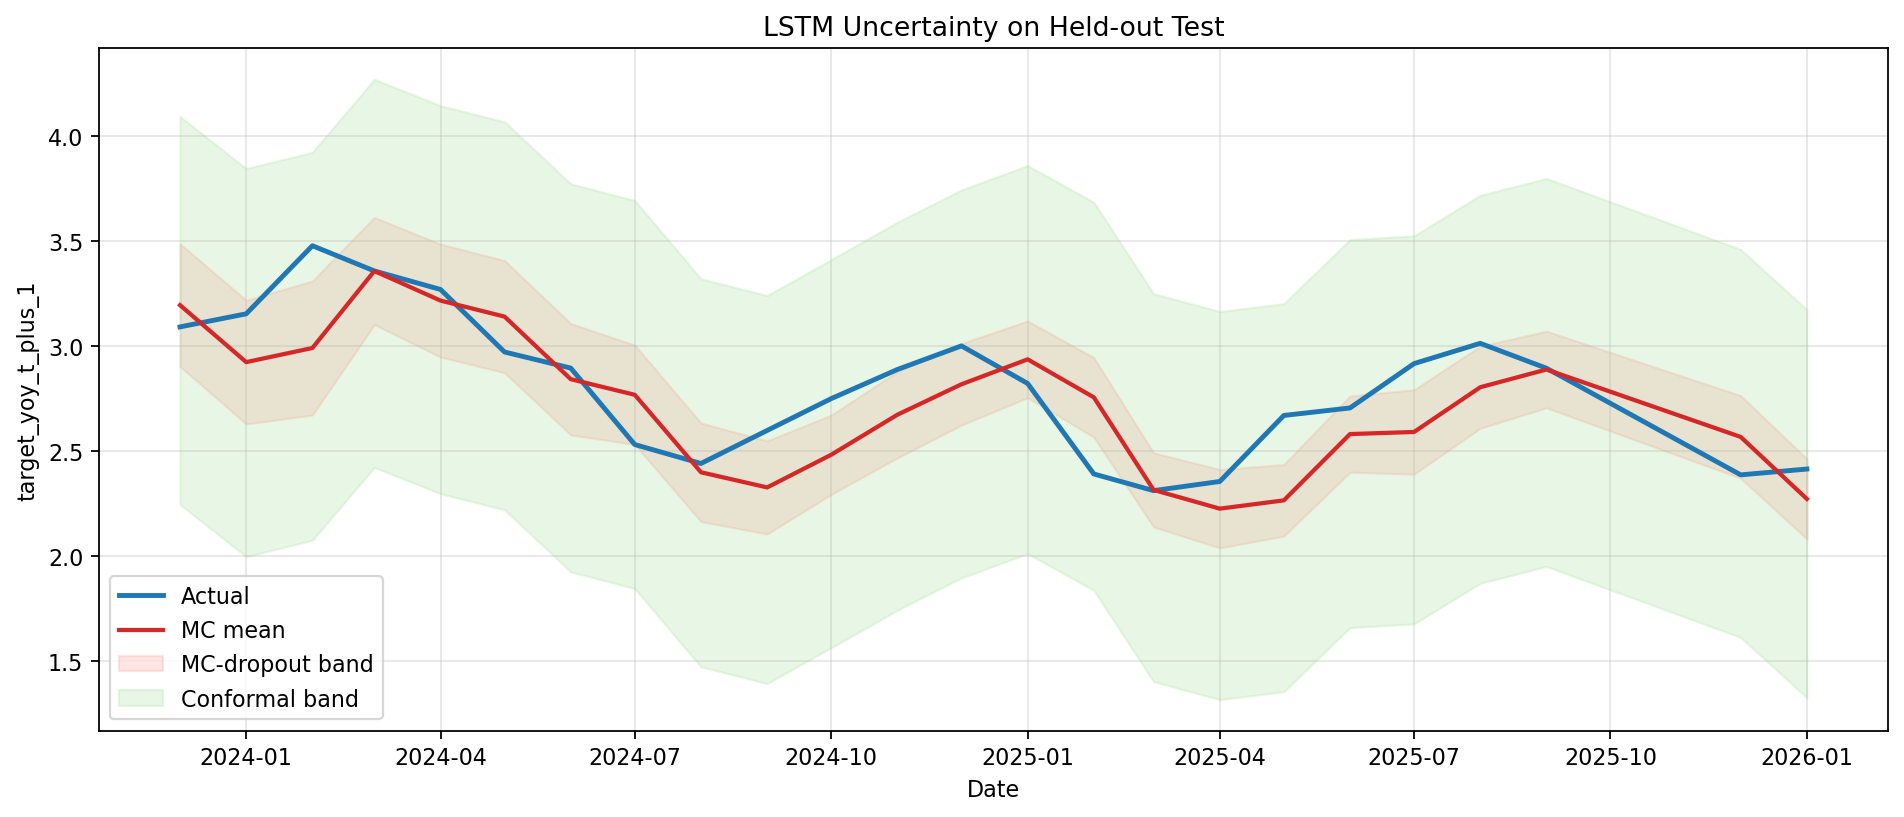
\includegraphics[width=0.74\textwidth]{figures/uncertainty_intervals.png}
\caption{LSTM uncertainty intervals.}
\end{figure}

\begin{figure}[H]
\centering
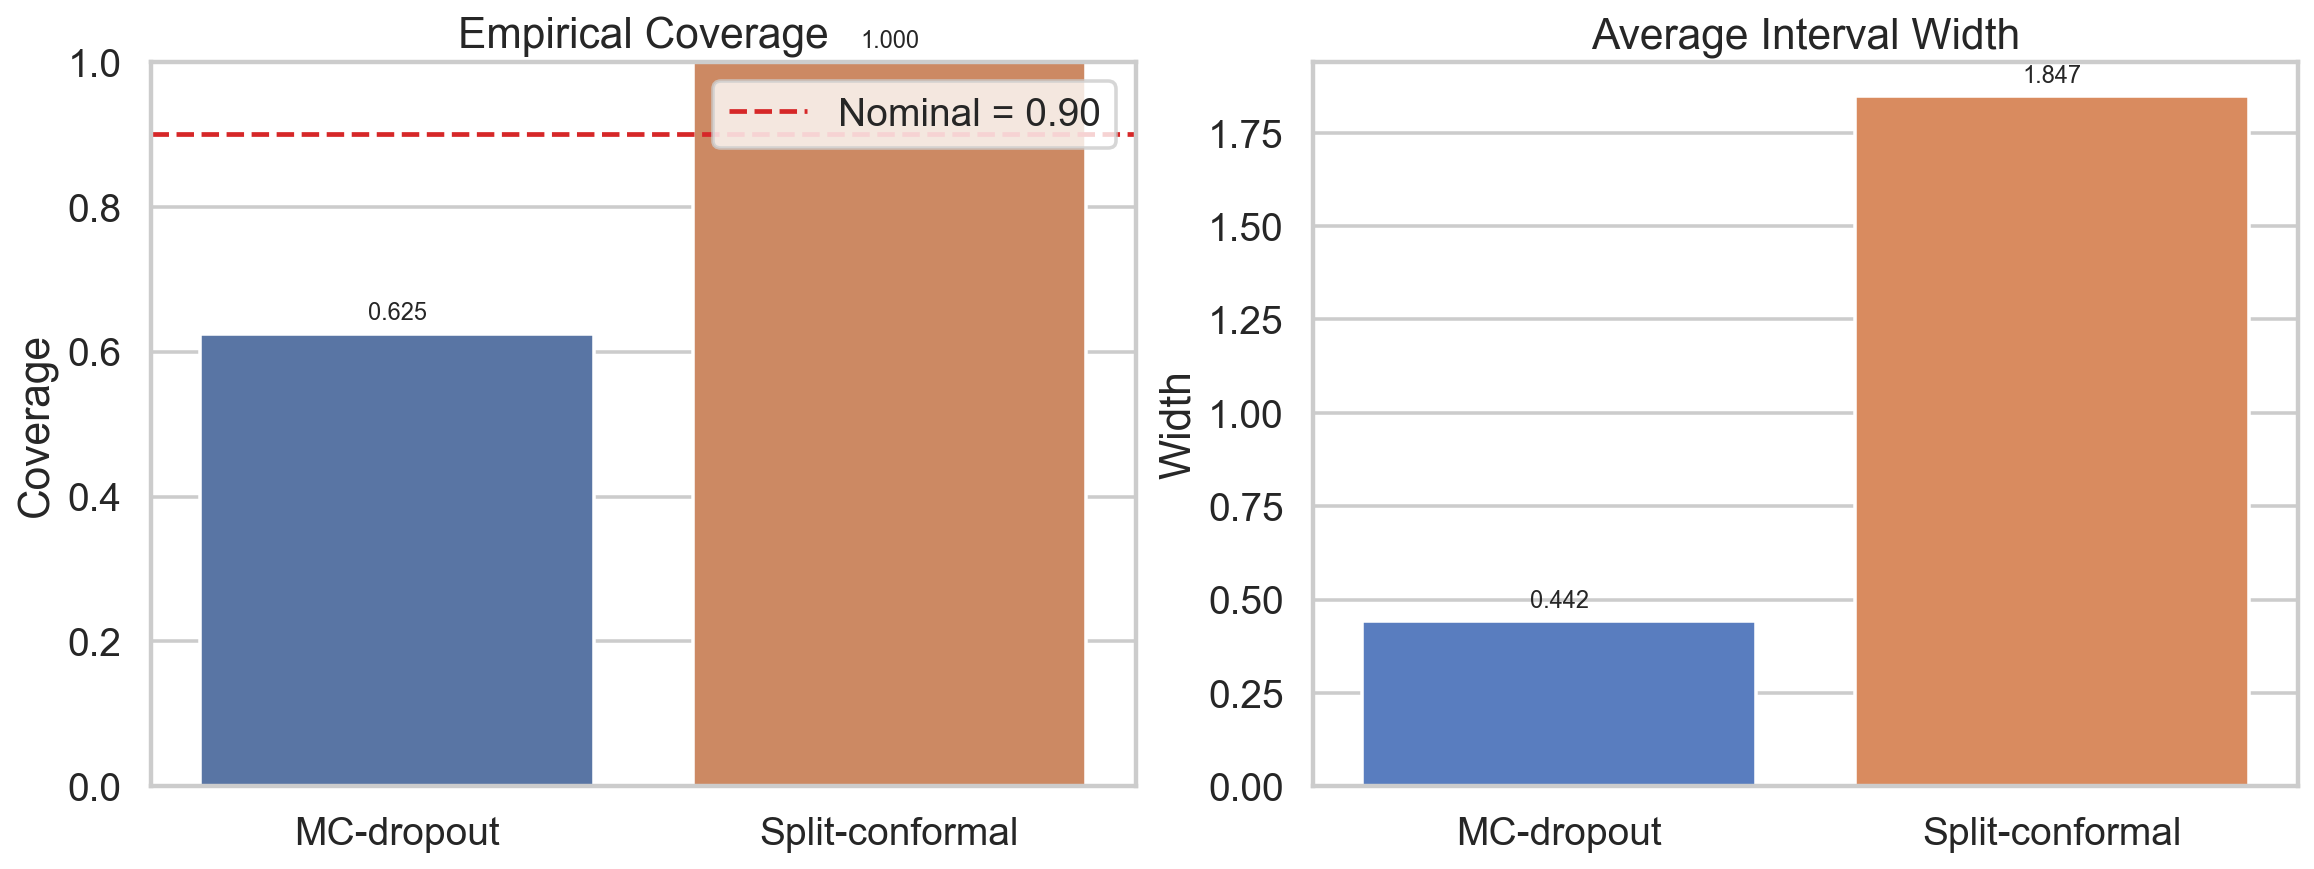
\includegraphics[width=0.62\textwidth]{figures/uncertainty_coverage_summary.png}
\caption{Coverage versus nominal target.}
\end{figure}

Extra diagnostic: both sequence and tree predictions show a small timing lag in this test window.
For unshifted predictions, MAE is 0.1787 (LSTM) and 0.1584 (XGBoost).
If predictions are shifted by one month, MAE drops to 0.1063 (LSTM) and 0.0498 (XGBoost), so the lag pattern is visible in both models.

\begin{figure}[H]
\centering
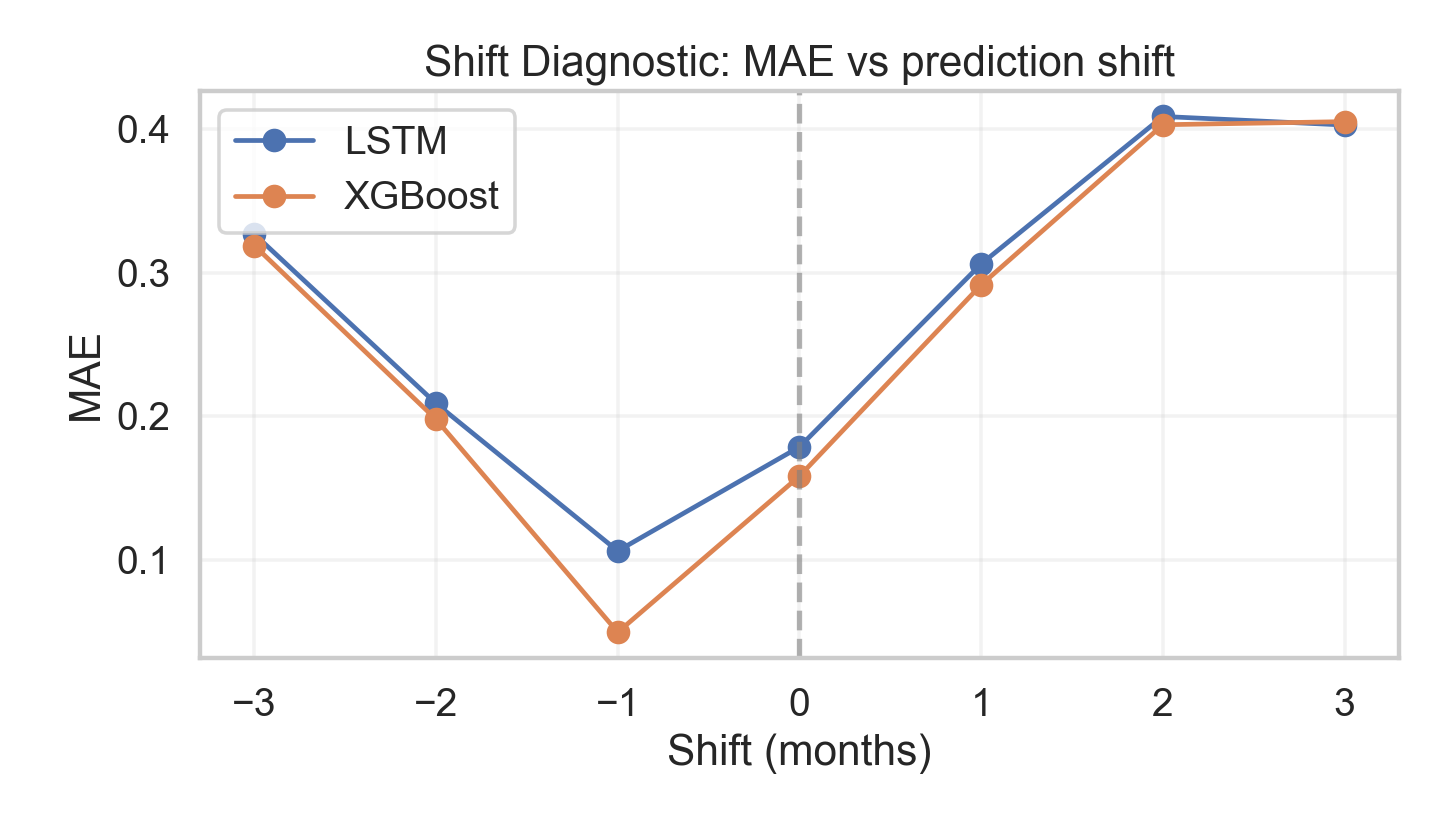
\includegraphics[width=0.74\textwidth]{figures/lag_shift_mae_by_model.png}
\caption{Shift diagnostic: MAE under temporal shifts for LSTM and XGBoost.}
\end{figure}

\begin{figure}[H]
\centering
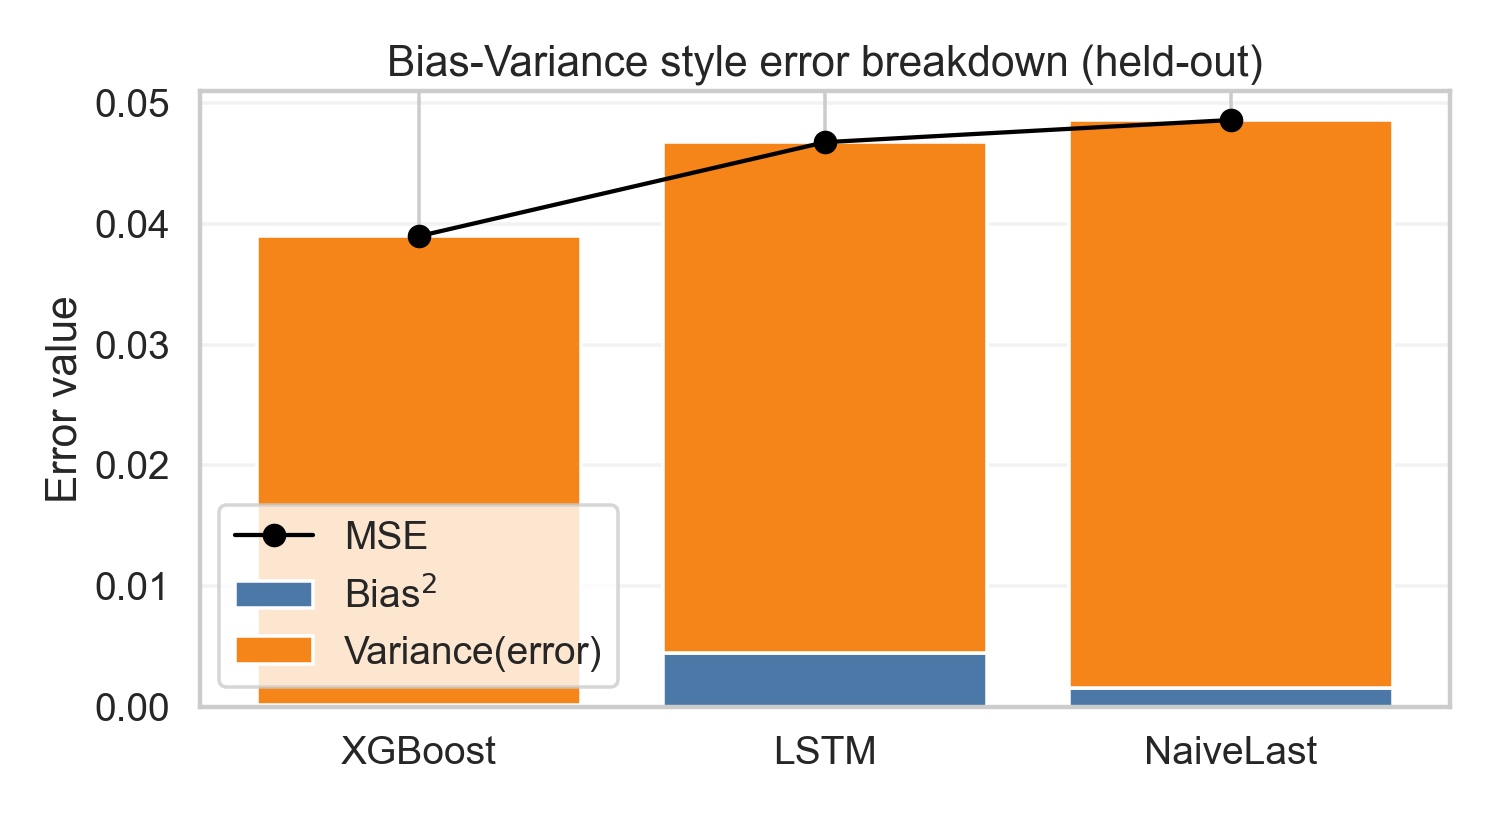
\includegraphics[width=0.74\textwidth]{figures/bias_variance_error_breakdown.png}
\caption{Bias-variance style error decomposition on held-out test.}
\end{figure}

\section{Conclusions}
\begin{enumerate}
  \item XGBoost is the strongest final model on the shared held-out benchmark.
  \item Lasso is a strong and simple baseline close to the winner.
  \item LSTM learned general movement but did not beat XGBoost and showed slight timing delay around turning points.
  \item Performance varies by macro regime in rolling windows, so one fixed score does not tell the full story.
  \item Interval calibration still needs improvement for practical risk bounds.
  \item Overall, for this monthly macro setup, careful feature engineering plus tree models gave the best accuracy-cost tradeoff.
  \item Next step would be to improve turning-point timing and re-calibrate uncertainty intervals.
\end{enumerate}

\end{document}
